\section{Estado del arte y antecedentes}

\subsection{Estado del arte del problema a tratar}

El problema de la estimación de la edad a partir de restos óseos ya se ha tratado en distintas ocasiones, desde modificaciones a la propuesta de Todd, propuestas de como automatizar la estimación utilizando las características que proponía Todd, hasta estudios que utilizaban técnicas de visión por computador para recoger y procesar las características de los restos.

En 1990, J. M. Suchey y S. Brooks propusieron una modificación a la propuesta de Todd \cite{sucheyBrooks}, en la que evaluaban $1225$ restos óseos y llegaban a la conclusión de que era posible reducir las diez fases propuestas por Todd a seis fases, modificando el criterio de cada una de las fases y añadiendo cierto error marginal, aunque con un $95\%$ de confianza con los nuevos intervalos propuestos. Esta modificación es una de las más aceptadas por la comunidad científica, aunque la mayor parte de trabajos siguen utilizando las fases propuestas por Todd.

Uno de los más relevantes es un estudio publicado en el año 2015 en la revista \textit{Journal of forensic sciences} \cite{modelandoHuesos3D}, en el que se escaneaban los restos tomados como muestras para la variación de la sínfisis púbica y con esta variación realizar la estimación de la edad utilizando un modelo de regresión lineal y las seis fases propuestas por Suchey y Brooks. El conjunto de datos utilizado en este experimento se compone de $41$ esqueletos de personas estadounidenses y logran obtener una raíz del error cuadrático medio de unos $17.15$ años.

\begin{figure}[H]
	\centering
	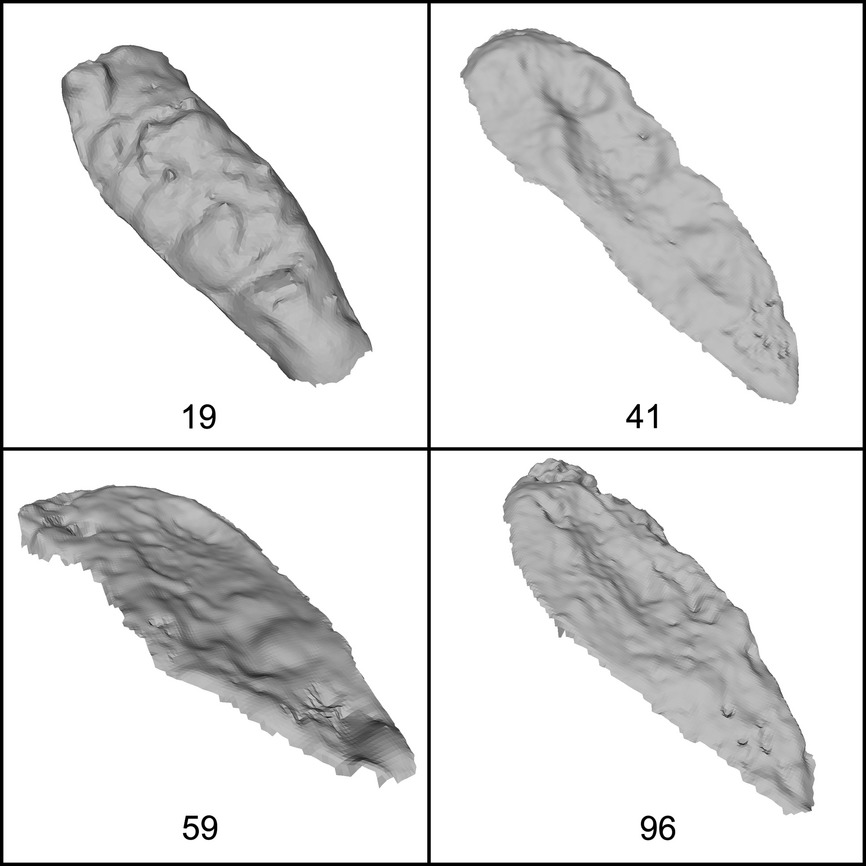
\includegraphics[scale = 0.4]{escaneo_huesos.jpg}
	\caption{Visualización del escaneo de la sínfisis púbica en cuatro individuos. La edad de la muerte aparece en la parte inferior de cada imagen. Imagen obtenida de \cite{modelandoHuesos3D}.}
	\label{fig:escaneo_huesos}
\end{figure}

Ese mismo año, los mismos autores presentaron una mejora \cite{mejoraModelandoHuesos3D} en la que, en lugar de utilizar la variación total de la sínfisis púbica, utilizaban la flexión de un plano de forma que dicho plano coincida con la superficie del hueso. De esta forma, utilizando un conjunto de datos similar a su experimento anterior y la curvatura de la sínfisis púbica entrenaron un modelo de regresión lineal con el que obtuvieron una raíz del error cuadrático medio de unos $19$ años.

A finales de 2015, Beatrix Dudzik y Natalie R. Langley, de la Universidad de Tennessee y la Universidad Lincoln Memorial, propusieron \cite{componentBased} varios modelos basados en árboles de decisión y regresión logística multinomial. Para estos experimentos utilizaron 5 características de la sínfisis púbica de 47 individuos de entre 18 y 40 años. Obtuvieron muy buenos resultados, con una tasa de acierto del $94\%$ aunque solo utilizaban 3 de las 6 fases propuestas por Suchey y Brooks.

\begin{figure}[H]
	\centering
	\begin{subfigure}{.5\textwidth}
	  \centering
	  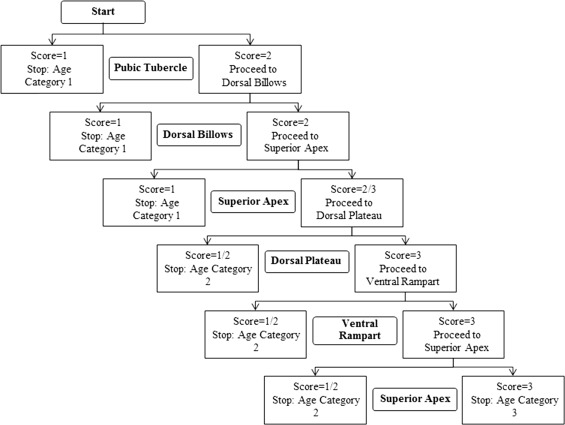
\includegraphics[scale = 0.8]{cita_7_arbol.jpg}
	  \caption{Árbol de decisión implementado en \cite{componentBased}}
	  \label{fig:arbol_c7}
	\end{subfigure}%
	\begin{subfigure}{.5\textwidth}
	  \centering
	  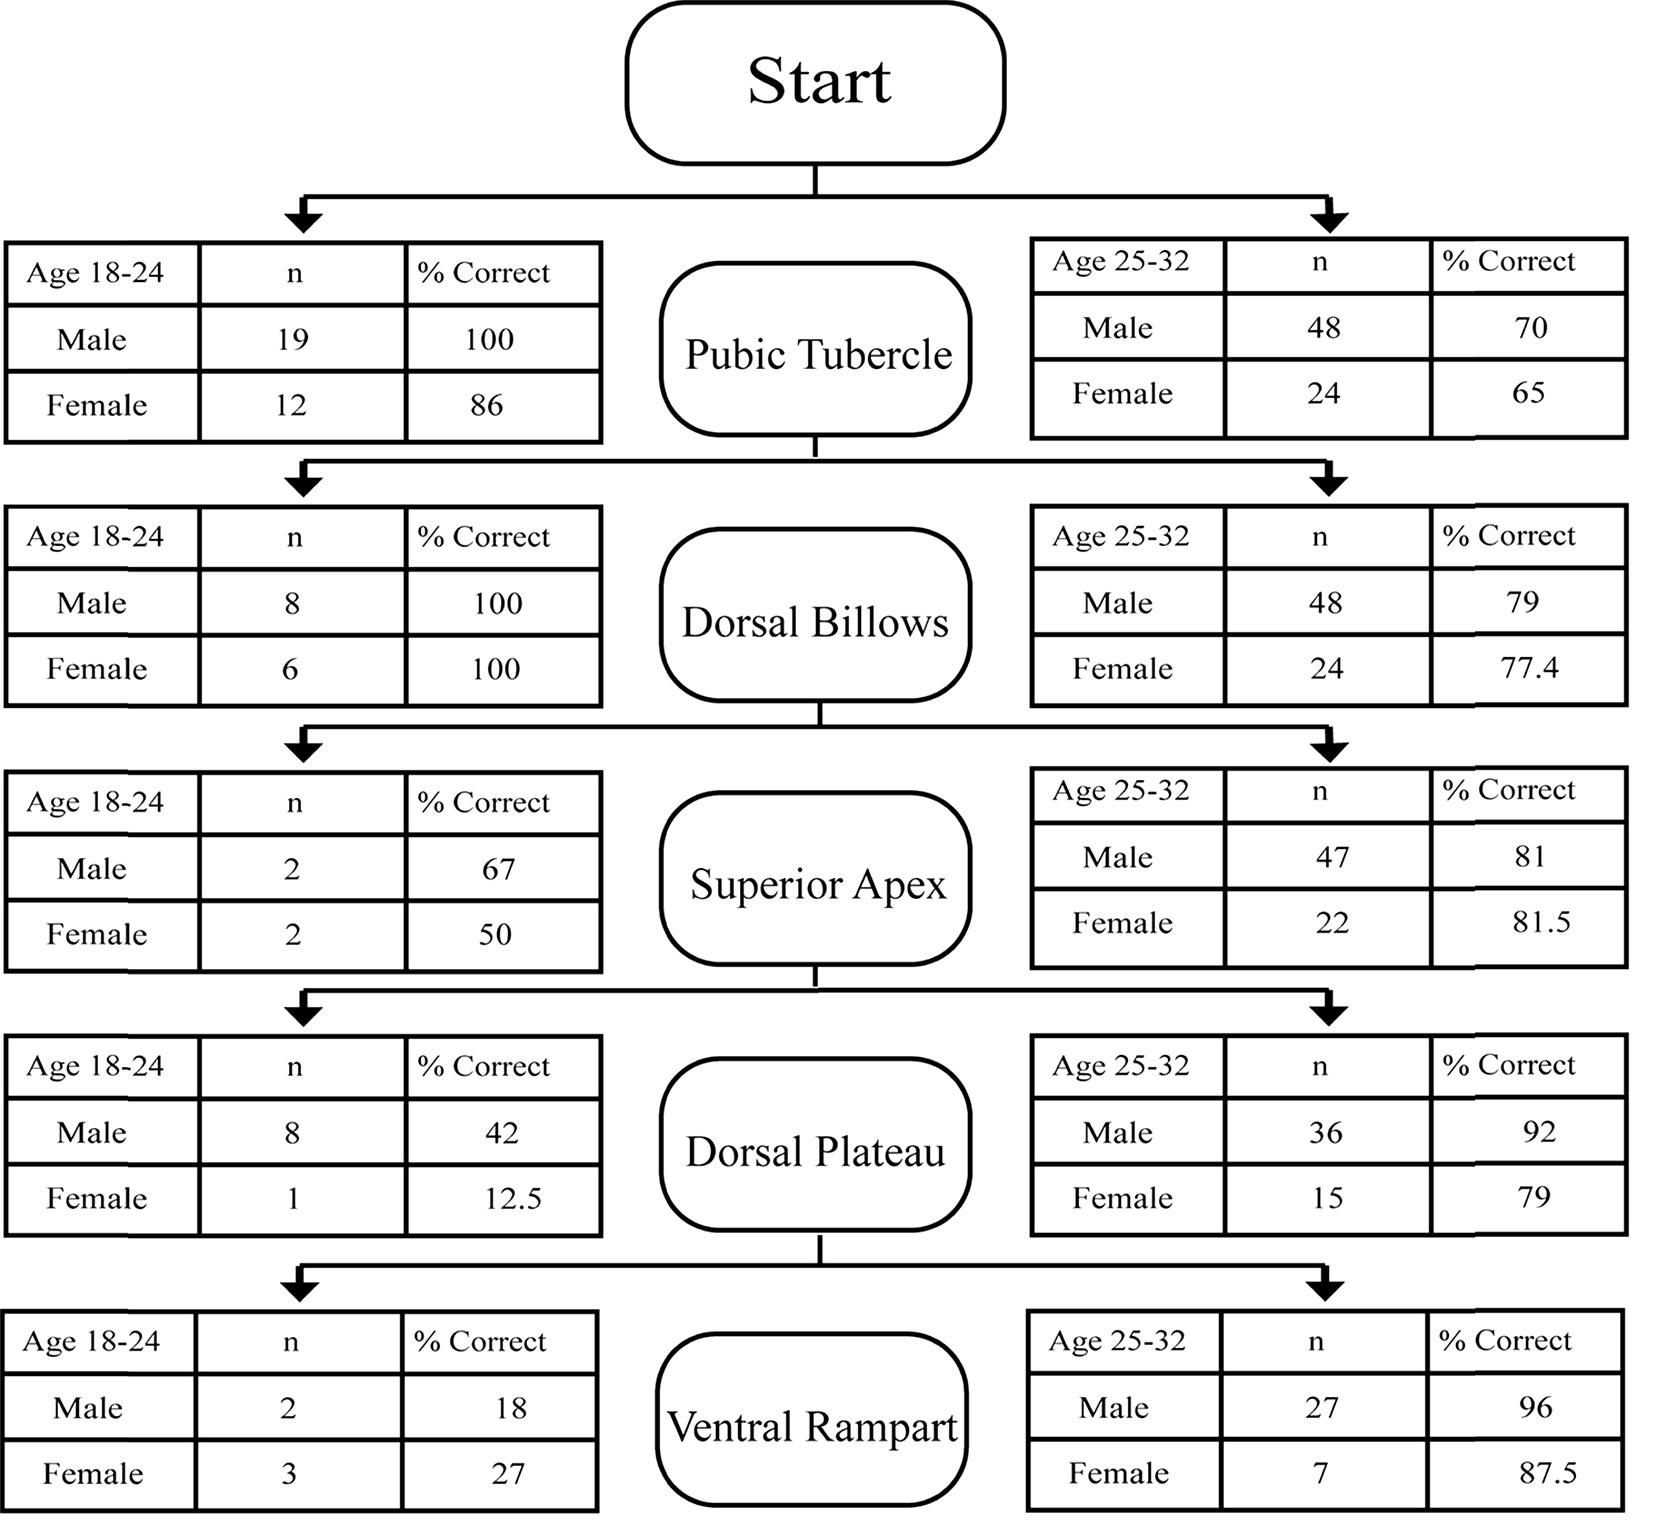
\includegraphics[scale = 0.8]{cita_7_ejemplo_dos_fases.jpg}
	  \caption{Porcentaje de acierto para la fase 1 y 2 de \cite{componentBased}.}
	  \label{fig:acierto_cita7}
	\end{subfigure}
	\caption{Imágenes obtenidas de \cite{componentBased}.}
	\label{fig:arboles_cita7}
\end{figure}



Más adelante, en 2018, varios investigadores de la República Checa publicaron un trabajo \cite{estimacionHuesosCadera} en el que, con un conjunto de $941$ restos óseos de personas de distinta raza entre 19 y 100 años, utilizando datos de los huesos de la cadera estudiaban las características comunes y las que diferenciaban las distintas edades, y consideraban 9 modelos distintos para realizar una estimación, desde un sistema de puntuación tradicional, utilizando la variación entre los huesos, distintos de regresión lineal, árboles de decisiones o redes neuronales artificiales. De estos modelos se llega a la conclusión que el mejor es un modelo de regresión multinomial, con el que obtienen una raíz del error cuadrático medio de unos $12.5$ años.

En 2017 investigadores de la Universidad de Granada publicaron un artículo preliminar de cara a obtener un modelo descriptivo basado en reglas con el que realizar la estimación de la edad a partir de la sínfisis púbica \cite{fuzzyAgeEstimation}. Utilizando $74$ muestras clasificadas manualmente consiguen entre 17 y 20 reglas utilizando árboles de decisión difusos que consiguen un error absoluto medio de $1.68$ años, aunque el resultado no es totalmente fiable debido a que no consiguen reglas para algunas fases propuestas por Todd.

Más adelante, en 2021, este mismo equipo con la ayuda de investigadores de la Universidad de Cordoba publicaron una continuación de su estudio \cite{NSLVOrdAge}. En este caso, utilizando el mismo conjunto de datos que utilizaremos nosotros, aplicando técnicas de balanceo y sobremuestreo de datos para resolver problemas relativos a dicho conjunto de datos, han enfocado el problema como un problema de clasificación ordinal. Utilizando el software NSLVOrd \cite{NSLVOrd}, un algoritmo de clasificación ordinal basado en el enfoque de aprendizaje de reglas de forma iterativa publicado por investigadores de la Universidad de Granada en 2016, son capaces de obtener una raíz del error cuadrático medio de $12.34$ años utilizando 34 reglas para las distintas fases. Este es, hasta este momento, el mejor resultado del estado del arte de este problema, y además en este estudio se discute sobre la importancia de las características a observar en la sínfisis púbica propuestas por Todd, llegando a la conclusión de que ciertas características nunca se utilizan, y por lo tanto no entran en juego a la hora de realizar la estimación de la edad.

\subsection{Programación Genética y regresión simbólica}

La Programación Genética apareció como una adaptación de los algoritmos genéticos para representar programas de ordenador como cromosomas en una estructura de árbol. A pesar de que su aparición fue en 1985 no fue hasta principios de 1990 cuando este método comenzo a ser más utilizado gracias a John Koza \cite{kozaGP}.

La forma en la que la Programación Genética expresa los cromosomas permite resolver problemas de distintos tipos dando soluciones sencillas de interpretar, por este motivo este algoritmo y sus variaciones han sido bastante utilizadas.

Uno de los primeros trabajos fue de publicado por P. A. Whigham en 1995 \cite{PGgramaticas}, en el que se proponía utilizar una gramática inicial libre del contexto para generar expresiones a utilizar en el algoritmo de Programación Genética, y que el entrenamiento del algoritmo fuera capaz de completar la gramática y ampliándola con nuevas reglas, siendo un claro ejemplo de aprendizaje incremental.

Ese mismo año investigadores de la Universidad de Georgia publicaban un artículo \cite{primerGAP} en el que proponían utilizar Programación Genética para hacer regresión simbólica, es decir, aprender una fórmula matemática estructurada como un árbol, en este trabajo se mencionan los principales problemas de Programación Genética para ser aplicada a regresión simbólica y por eso se propone una modificación del algoritmo original, que será un híbrido entre Programación Genética y un Algoritmo Genético, de ahí el nombre GA-P (Genetic Algorithm-Programming).


Más adelante esta variación de Programación Genética se utilizará en diversos artículos, como el publicado por investigadores de la Universidad de Oviedo y la Universidad de Granada en 1999 \cite{GAPredElectrica}, donde utilizando este algoritmo consiguen unos resultados bastante buenos en dos problemas reales aplicando regresión simbólica.

Un año más tarde, en el año 2000, aunque ya se podían encontrar trabajos en los que se utilizaba Programación Genética y algunas variantes de cara a realizar regresión simbólica, dos investigadores del Laboratorio Nacional de Computación Científica de Brasil publican un artículo \cite{PGregresionSimbolica} donde explican como utilizar Programación Genética en regresión simbólica, explicando los distintos operadores necesarios.

En el año 2000, también investigadores de la Universidad de Granada, publicaron un trabajo donde utilizan GA-P para aprender consultas booleanas \cite{GAPFormulasBooleanas} en el que demuestran la versatilidad del algoritmo para distintos problemas, además de que las soluciones obtenidas son fácilmente interpretables.


%\subsection{Sistemas basados en reglas}


\newpage
